\documentclass[12pt,a4paper]{article}

% idioma e codificacao
\usepackage[utf8]{inputenc}
\usepackage[T1]{fontenc}
\usepackage[brazil]{babel}

% formatacao
\usepackage{geometry}
\usepackage{setspace}
\usepackage{indentfirst}
\usepackage{array}
\usepackage{tabularx}
\usepackage{hyperref}
\usepackage{enumitem}
\usepackage{graphicx}
\usepackage{float}
\usepackage{tabularx}
\usepackage{booktabs}
\usepackage[table]{xcolor}
\usepackage{tikz}

% Cores personalizadas
\definecolor{verdeFundo}{HTML}{E1F4EB}
\definecolor{verdeTexto}{HTML}{00823B}
\definecolor{vermelhoFundo}{HTML}{FBE7E9}
\definecolor{vermelhoTexto}{HTML}{B4232C}
\definecolor{cinzaLinha}{HTML}{D8DEDC}

% Badge arredondado
\newcommand{\badge}[3]{%
	\tikz[baseline=(texto.base)]{
		\node[
		fill=#1,
		text=#2,
		rounded corners=8pt,
		inner xsep=7pt,
		inner ysep=4pt,
		font=\sffamily\bfseries\scriptsize
		] (texto) {#3};
	}%
}

% Badges de permissão
\newcommand{\permitido}{%
	\badge{verdeFundo}{verdeTexto}{Permitido}%
}

\newcommand{\negado}{%
	\badge{vermelhoFundo}{vermelhoTexto}{Negado}%
}

\geometry{
top=3cm,bottom=2cm,left=3cm,right=2cm}

\onehalfspacing
\setlength{\parindent}{1,25cm}
\setlength{\parskip}{0.3em}

\hypersetup{
	colorlinks=true,
	urlcolor=blue,
	linkcolor=black
}

\begin{document}

% IDENTIFICACAO
\begin{center}
	{\large \textbf{Atividade de Reposição de Aula}}\\
	\vspace{0.5cm}
	\textbf{Segurança em Microserviços com Spring Security}\\
\end{center}

\vspace{0.7cm}

\noindent
\textbf{Aluno:} Gabriel Victorino\\
\textbf{Turma:} SEXTO SEMESTRE\\
\textbf{Disciplina:} LABORATÓRIO DE DESENVOLVIMENTO MULTIPLATAFORMA\\
\textbf{Data:} \today

\vspace{0.5cm}	

\section{Introdução}
	A arquitetura de microsserviços permite criar um aplicativo com uma estrutura de componentes, independentes entre si, executando processos como serviço. Cada componente possui atuação e objetivos únicos, com a implantação, escalabilidade e atualização de cada um, sendo gerenciada separadamente.


\section{Autenticação e Autorização}
Autenticação é quando as credenciais informadas são validadas no sistema, como a senha/token utilizado ao realizar o login no sistema. Quando falamos de autorização, estamos falando de quais arquivos acessamos, ou seja, quais ações o perfil do usuário logado pode acessar, como um acesso somente leitura.

Para os exemplos, a autenticação é validação do token na api e autorização seria ao acessar o recurso de DELETE /product-composite/{productId}.

\section{Proteção das Requisições}
A SecurityFilterChain é responsável por definir como as requisições HTTP serão protegidas pelo Spring Security. Antes de uma requisição chegar ao controller, ela passa por uma cadeia de filtros que pode verificar credenciais, identificar o usuário autenticado, tratar falhas de segurança e avaliar se ele possui permissão para acessar a operação solicitada.

\begin{figure}[H]
	\centering
	\setlength{\fboxrule}{1pt}
	\setlength{\fboxsep}{2pt}
	 \fbox{
		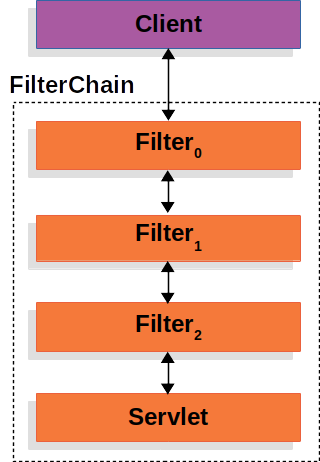
\includegraphics[width=0.3\textwidth]{./filterchain.png}
	}
	\caption{Filter Chain}
	\label{fig:filterchain}
\end{figure}


As regras de segurança podem considerar a rota solicitada, o método HTTP e os papéis atribuídos ao usuário. No workshop-microservices, por exemplo, uma regra poderia permitir que usuários LEITOR e ADMIN consultassem um produto agregado, enquanto somente o ADMIN poderia criar ou excluir produtos. Quando uma requisição chega, o Spring Security encontra a regra correspondente e compara suas exigências com a autenticação e as permissões do usuário.

Se os requisitos forem atendidos, a requisição segue para a operação. Caso contrário, o acesso é recusado. Uma requisição sem autenticação válida normalmente recebe a resposta 401 Unauthorized, enquanto um usuário autenticado sem a permissão necessária recebe 403 Forbidden.

\section{Política de Acesso}


\begin{table}[htbp]
	\centering
	\renewcommand{\arraystretch}{1.8}
	\setlength{\tabcolsep}{6pt}
	
	\begin{tabularx}{\textwidth}{
			>{\raggedright\arraybackslash}X
			>{\centering\arraybackslash}p{2.6cm}
			>{\centering\arraybackslash}p{2.6cm}
			>{\centering\arraybackslash}p{2.6cm}
		}
		
		\textbf{OPERAÇÃO} &
		\textbf{VISITANTE} &
		\textbf{LEITOR} &
		\textbf{ADMIN} \\
		
		\arrayrulecolor{cinzaLinha}
		\midrule
		
		Consultar produtos (\texttt{GET}) &
		\permitido & \permitido & \permitido \\
		
		\midrule
		
		Criar produto (\texttt{POST}) &
		\negado & \negado & \permitido \\
		
		\midrule
		
		Excluir produto (\texttt{DELETE}) &
		\negado & \negado & \permitido \\
		
		\bottomrule
		
	\end{tabularx}
	
	\caption{Política de acesso aos produtos}
	\label{tab:permissoes}
\end{table}

O visitante sem autenticação não pode acessar nenhuma operação, pois o sistema não consegue confirmar sua identidade. Essa decisão também evita a exposição pública dos dados dos produtos do workshop.

O usuário LEITOR pode consultar produtos, pois sua função é acessar informações sem modificá-las. Ele não pode criar nem excluir produtos, já que essas operações alteram os dados do sistema.

O usuário ADMIN pode consultar, criar e excluir produtos porque é responsável pela administração dos recursos. A exclusão exige atenção especial, pois também pode remover informações relacionadas ao produto.

Essa política segue o princípio do menor privilégio: cada usuário recebe somente as permissões necessárias para exercer sua função. Assim, operações de leitura são disponibilizadas aos usuários autenticados, enquanto alterações ficam restritas ao administrador.

\section{Cenários de Acesso}
Quando uma requisição chega a uma operação protegida sem credenciais, a API deve responder com 401 Unauthorized. Essa resposta informa que o cliente precisa se autenticar para acessar o recurso.

Quando as credenciais são inválidas, expiradas ou não podem ser verificadas, a resposta também deve ser 401 Unauthorized. Nesse caso, a autenticação não foi concluída e, portanto, o sistema não reconhece uma identidade válida.

Quando o usuário está autenticado, mas não possui a permissão exigida, a API deve responder com 403 Forbidden. Por exemplo, um usuário LEITOR que tente excluir um produto deve receber 403, pois sua identidade foi reconhecida, mas seu papel não permite essa operação.

Portanto, 401 significa que não existe uma autenticação válida, enquanto 403 significa que o usuário foi autenticado, mas não está autorizado a executar a ação solicitada. A apresentação de credenciais válidas pode resolver um erro 401; para resolver um 403, é necessário que o usuário receba a permissão adequada.

\section{Decisão de Arquitetura}

Se cada microserviço mantivesse seu próprio cadastro de usuários e senhas, um dos principais problemas seria a duplicação e a inconsistência dos dados. Uma mesma pessoa poderia possuir registros diferentes em vários serviços. A alteração de uma senha, permissão ou situação da conta teria de ser repetida em todos eles. Caso alguma atualização falhasse, um usuário bloqueado poderia continuar acessando parte do sistema.

Outro problema seria o aumento da superfície de ataque. Cada microserviço teria de armazenar e proteger senhas, além de implementar corretamente recursos como criptografia, recuperação de conta, bloqueio por tentativas e auditoria. Uma falha de segurança em apenas um serviço poderia expor as credenciais dos usuários.

Também haveria maior dificuldade de manutenção e uma experiência ruim para o usuário, que poderia precisar utilizar credenciais diferentes em cada serviço. Uma abordagem mais adequada seria centralizar a autenticação em um serviço de identidade. Dessa forma, os microserviços validariam a identidade recebida e continuariam responsáveis apenas por verificar as permissões necessárias para suas próprias operações.

\section*{Referências}
\addcontentsline{toc}{section}{Referências}

\begin{enumerate}[leftmargin=*]

\item F290-LDMP
\textbf{Workshop Microservices}
Github. Disponível em:
\url{https://github.com/F290-LDMP/workshop-microservices}

\item Amazon
\textbf{Microsserviços}
Crie microsserviços altamente disponíveis como base para aplicações de qualquer porte e escala. Disponível em:
\url{https://aws.amazon.com/pt/microservices/}

\item Spring Security
\textbf{Arquitetura}
Disponível em:
\url{https://docs.spring.io/spring-security/reference/servlet/architecture.html}

\end{enumerate}

\end{document}